\section{Interpolating Curve Planners} \label{C. Interpolating curve planners}

% \todo{Add more citations}

The algorithms that lie into this section are used in the local planning part of the pathfinding problem. They attempt to find a trajectory that fits a given global description of the path (such as way-points) by taking into account multiple parameters such as feasibility, comfort, vehicle dynamics and efficiency. Interpolation is used to increase the number of data points between the way-points in order to smooth out the trajectory and create easily traversable paths for non-holonomic robots \cite{gonzalez2016review}.

\textbf{Lines and Circles.} Primitives such as lines and circles can be used to describe the local path between two way-points. Figure \ref{fig:c_all_curve_planners}(a) represents the shortest path to execute a 3-step 180\degree turn for a car. Because it can only fit geometric primitives, the algorithm is simple to implement and fast, but it is also quite limited (preferential parameters such as curvature angle and continuation are completely ignored).

\textbf{Clothoid Curves.} The implementation of this algorithm is based on Fresnel integrals, and the resulting curves offer a smoother transition between different curvatures (such as between a straight line and a curve) than Lines and Circles (See Figure \ref{fig:c_all_curve_planners}(b)). The algorithm accounts for multiple constraints such as dynamic and physical vehicle limitations (e.g. steering wheel), thus making it more robust for non-holonomic robots such as a car. Moreover, the algorithm was used in the design of highways and railways.

\textbf{Polynomial Curves.} This type of curves are mainly used to satisfy different preferential parameters such as angle and curvature when drawing the trajectory between two way-points. The main advantage of using this method is that the preferential parameters determine the coefficients of the polynomial, and thus, it is much more flexible. Figure \ref{fig:c_all_curve_planners}(c) represents an example of using polynomial curves to change lanes.

\textbf{Bézier Curves.} This algorithm produces curves based on control points. The control points placement defines the curvature at the beginning and the end of the curve.  The significant advantage of this algorithm is that it has a low computational cost since the shape of the curve is defined by the control points. Therefore, the algorithm has been extensively used in different drawing software applications, technical drawing (they can also be drawn by hand) and trajectory design. Moreover, the curve can be used to approximate clothoid curves. Figure \ref{fig:c_all_curve_planners}(d) represents an example of using 3rd and 4th degree Béziers to find the best curvature estimate based on the current situation.

\textbf{Spline Curves.} The spline curve is sub-divided into multiple parametric patches that can be defined as polynomial curves, clothoid curves and b-splines (Bézier curves). Splines have a high degree of smoothness at each patch joint and can be extended into higher dimensions. Figure \ref{fig:c_all_curve_planners}(e) represents an example of a b-spline with a changing knot (the junction between two sub-segments).

It is worth mentioning that the global description of the path demands to include the collision-free areas in addition to the way-points or provide a collision detection system to be used when drawing the curves to ensure that no collisions are encountered while performing any of the above algorithms.

\begin{figure}[h!]
  \centering
  \begin{subfigure}[b]{0.22\linewidth}
    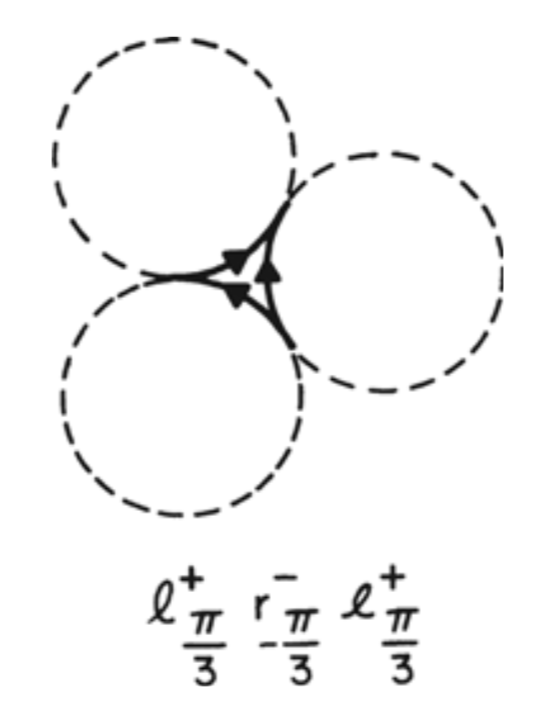
\includegraphics[width=\linewidth]{images/c_lines_and_circles.png}
     \caption{Lines and Circles \cite{gonzalez2016review}}
  \end{subfigure}
  \hfill
  \begin{subfigure}[b]{0.33\linewidth}
    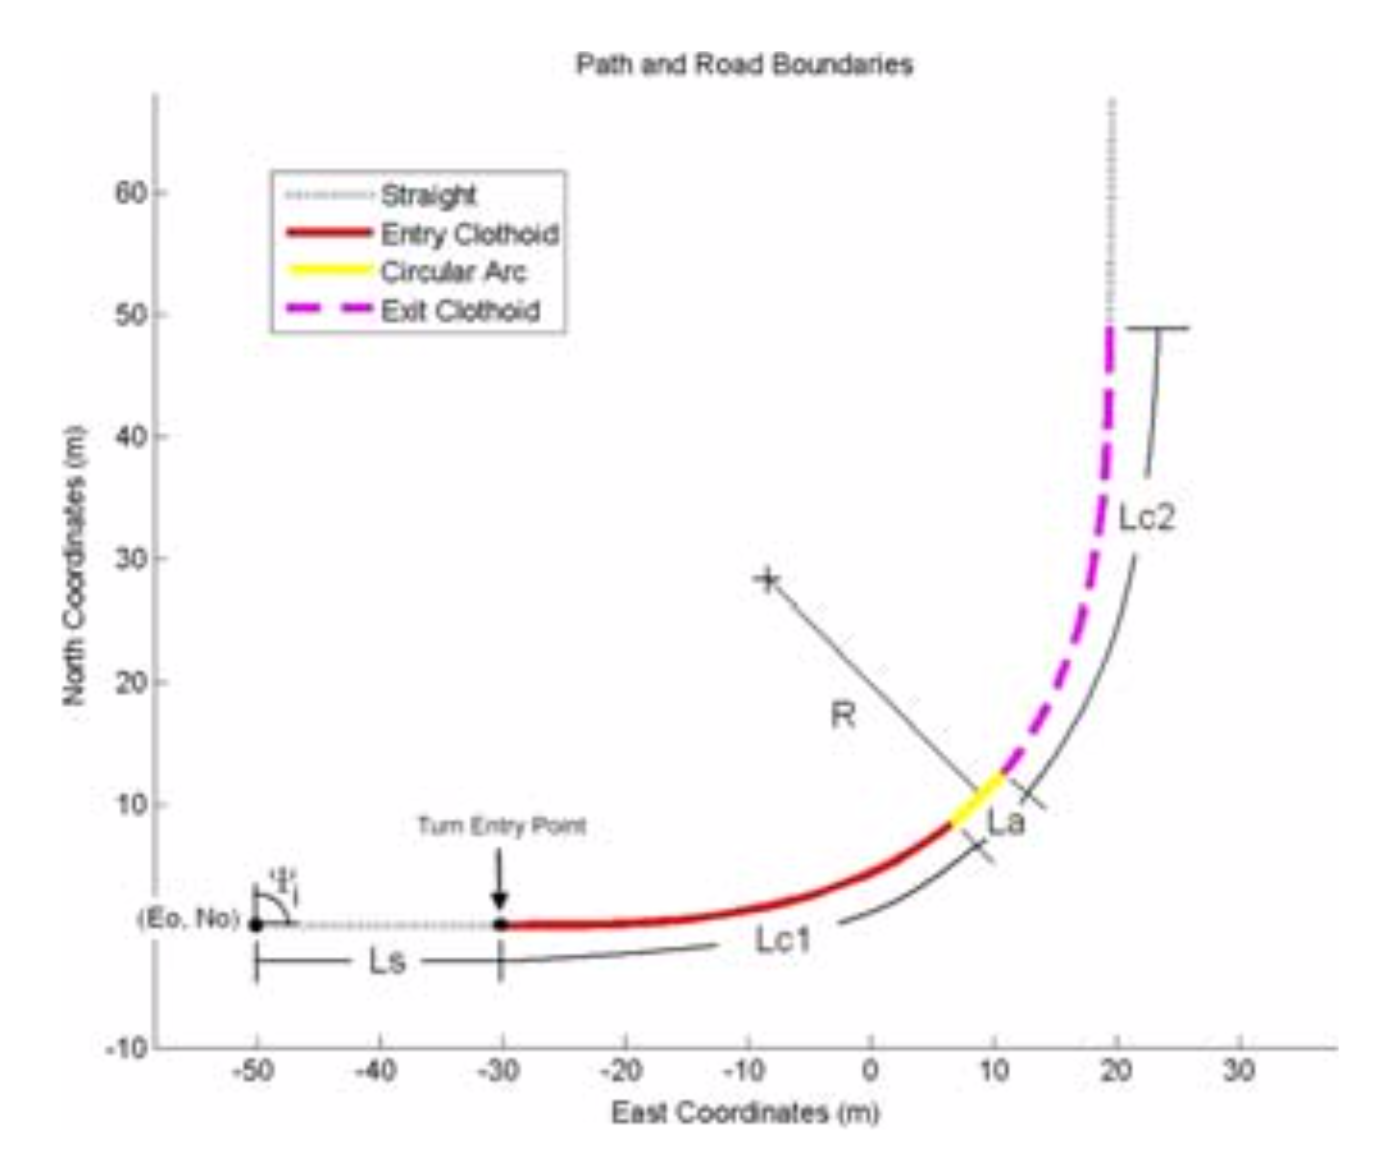
\includegraphics[width=\linewidth]{images/c_clothoid.png}
     \caption{Clothoid \cite{gonzalez2016review}}
  \end{subfigure}
  \hfill
  \begin{subfigure}[b]{0.38\linewidth}
    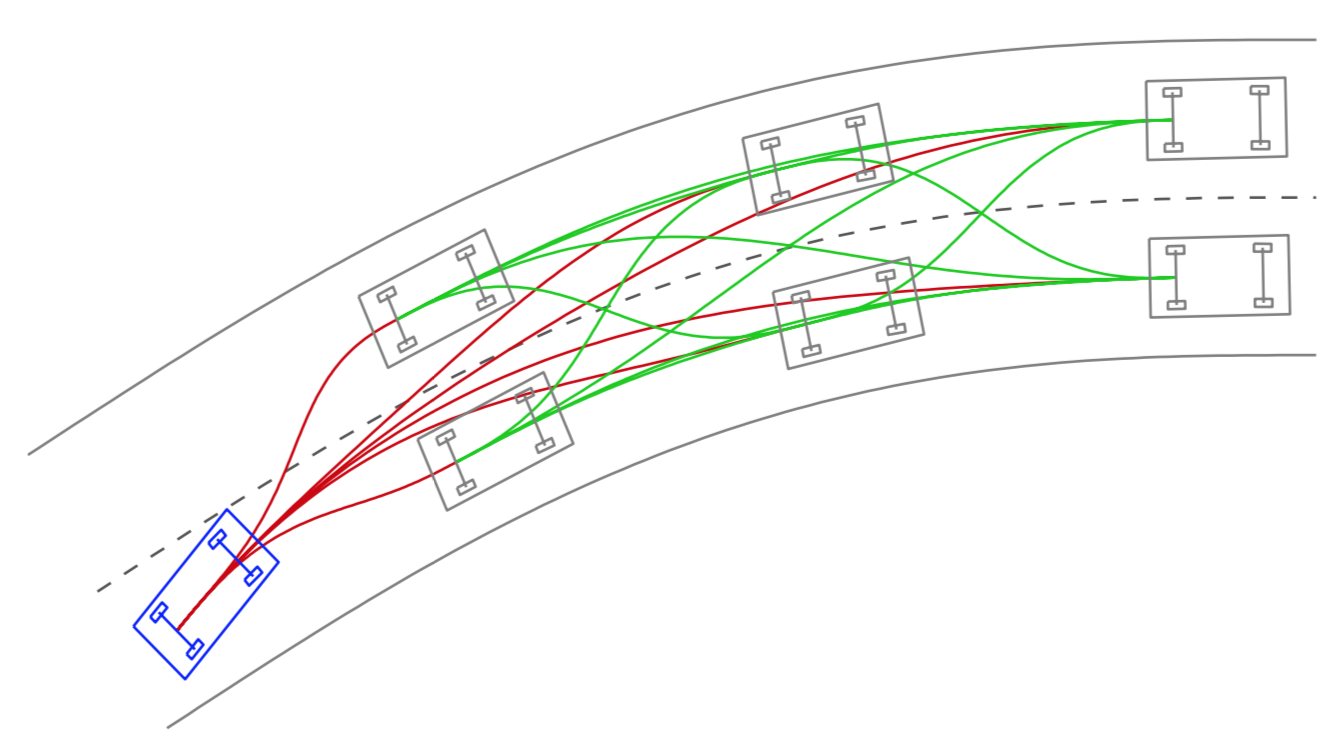
\includegraphics[width=\linewidth]{images/c_polynomial.png}
    \caption{Polynomial \cite{gonzalez2016review}}
  \end{subfigure}
  \newline
  \begin{subfigure}[b]{0.28\linewidth}
    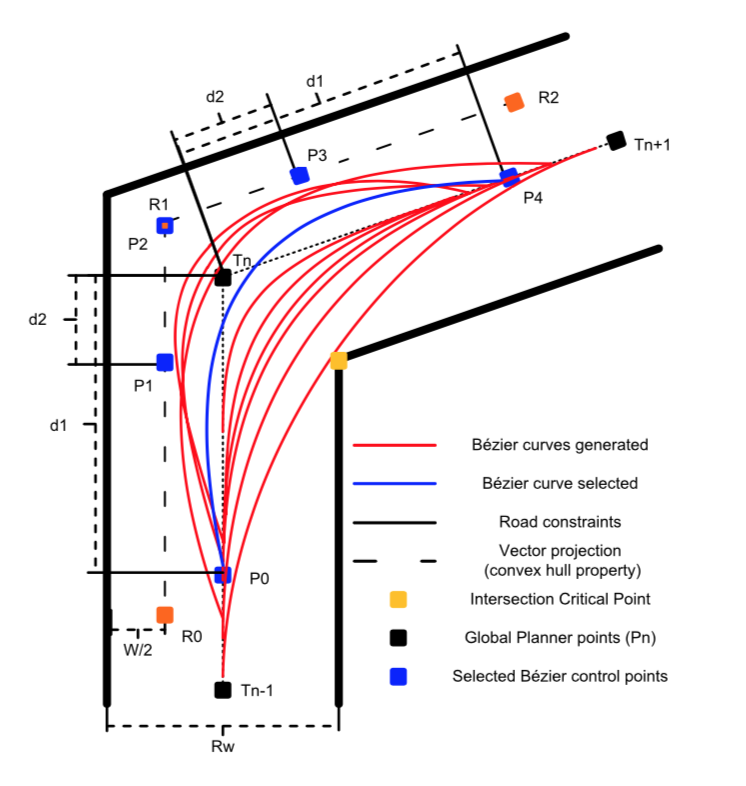
\includegraphics[width=\linewidth]{images/c_bezier.png}
     \caption{Bézier \cite{gonzalez2016review}}
  \end{subfigure}
  \hspace{1cm}
  \begin{subfigure}[b]{0.33\linewidth}
    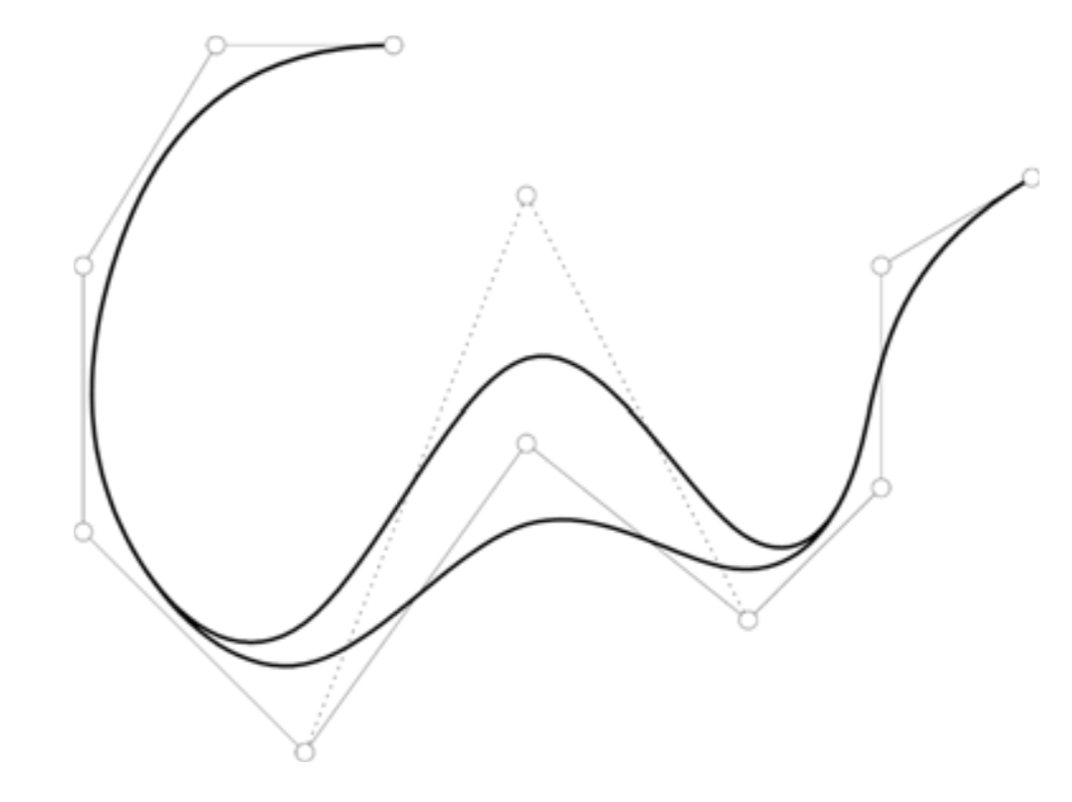
\includegraphics[width=\linewidth]{images/c_splines.png}
     \caption{Spline \cite{gonzalez2016review}}
  \end{subfigure}
  \caption{Examples of the most important interpolating curve planners}
  \label{fig:c_all_curve_planners}
\end{figure}